\setcounter{figure}{0}
\section{26th March 2023: Seven bowls of God's wrath}
\subsection*{Text: Revelation 15,16}
  \begin{quote}
    [1] Then I saw another sign in heaven, great and amazing, seven angels
    with seven plagues, which are the last, for with them the wrath of God is
    finished.

    [2] And I saw what appeared to be a sea of glass mingled with fire—and
    also those who had conquered the beast and its image and the number of
    its name, standing beside the sea of glass with harps of God in their
    hands.  [3] And they sing the song of Moses, the servant of God, and the
    song of the Lamb, saying,

    “Great and amazing are your deeds,
        O Lord God the Almighty!
    Just and true are your ways,
        O King of the nations!
    [4] Who will not fear, O Lord,
        and glorify your name?
    For you alone are holy.
        All nations will come
        and worship you,
    for your righteous acts have been revealed.”


    [5] After this I looked, and the sanctuary of the tent of witness in
    heaven was opened, [6] and out of the sanctuary came the seven angels
    with the seven plagues, clothed in pure, bright linen, with golden sashes
    around their chests.  [7] And one of the four living creatures gave to
    the seven angels seven golden bowls full of the wrath of God who lives
    forever and ever, [8] and the sanctuary was filled with smoke from the
    glory of God and from his power, and no one could enter the sanctuary
    until the seven plagues of the seven angels were finished.

    [1] Then I heard a loud voice from the temple telling the seven angels,
    “Go and pour out on the earth the seven bowls of the wrath of God.”

    [2] So the first angel went and poured out his bowl on the earth, and
    harmful and painful sores came upon the people who bore the mark of the
    beast and worshiped its image.

    [3] The second angel poured out his bowl into the sea, and it became like
    the blood of a corpse, and every living thing died that was in the sea.

    [4] The third angel poured out his bowl into the rivers and the springs
    of water, and they became blood.  [5] And I heard the angel in charge of
    the waters say,

    “Just are you, O Holy One, who is and who was,
        for you brought these judgments.
    [6] For they have shed the blood of saints and prophets,
        and you have given them blood to drink.
    It is what they deserve!”


    [7] And I heard the altar saying,

    “Yes, Lord God the Almighty,
        true and just are your judgments!”


    [8] The fourth angel poured out his bowl on the sun, and it was allowed
    to scorch people with fire.  [9] They were scorched by the fierce heat,
    and they cursed the name of God who had power over these plagues.  They
    did not repent and give him glory.

    [10] The fifth angel poured out his bowl on the throne of the beast, and
    its kingdom was plunged into darkness.  People gnawed their tongues in
    anguish [11] and cursed the God of heaven for their pain and sores.  They
    did not repent of their deeds.

    [12] The sixth angel poured out his bowl on the great river Euphrates,
    and its water was dried up, to prepare the way for the kings from the
    east.  [13] And I saw, coming out of the mouth of the dragon and out of
    the mouth of the beast and out of the mouth of the false prophet, three
    unclean spirits like frogs.  [14] For they are demonic spirits,
    performing signs, who go abroad to the kings of the whole world, to
    assemble them for battle on the great day of God the Almighty.  [15]
    (“Behold, I am coming like a thief!  Blessed is the one who stays awake,
    keeping his garments on, that he may not go about naked and be seen
    exposed!”) [16] And they assembled them at the place that in Hebrew is
    called Armageddon.

    [17] The seventh angel poured out his bowl into the air, and a loud voice
    came out of the temple, from the throne, saying, “It is done!” [18] And
    there were flashes of lightning, rumblings, peals of thunder, and a great
    earthquake such as there had never been since man was on the earth, so
    great was that earthquake.  [19] The great city was split into three
    parts, and the cities of the nations fell, and God remembered Babylon the
    great, to make her drain the cup of the wine of the fury of his wrath.
    [20] And every island fled away, and no mountains were to be found.  [21]
    And great hailstones, about one hundred pounds each, fell from heaven on
    people; and they cursed God for the plague of the hail, because the
    plague was so severe.

  \end{quote}
\subsection*{Notes}
\begin{itemize}
  \item{Chapter 6-16 of Revelation covers the three series of judgments and the interludes in between. Some recap:
  \begin{itemize}
    \item{Revelation is more of a letter than a book.  John wrote the letter
    to the seven churches to encourage the churches who were facing
    persecution and opposition and temptations, and the purpose was to ask
    them to remain firm in their commitment to God.  It was to remind them
    that Christ will come back soon to right all the wrongs that were
    happening to them.}
    \item{Since the genre of the letter is also apocalyptic, it is full of
    symbols and should not be taken literally.  The symbols and the visions
    are not just about the future, they are relevant to the entire church
    age. Maybe kind of in an ``already but not yet'' kind of way.}
    \item{The key to the chapters 6-16 is in chapters 4-5, which is the
    throne room vision of God and the Father.  In this vision, we see the
    phrase ``every creature'' giving praise to God.  But for the seven
    churches currently receiving the letter, this is currently not their
    reality.  The purpose of the three judgments would then be to judge and
    eradicate evil so that God's final purpose of universal worship will be
    fulfilled.}
    \item{The three judgments are neither linear nor cyclical, they are
    following the so-called ``modified linear approach'' (c.f Figure $1$ of
    26th February 2023 sermon).  As we can see, all three judgments end with
    the throne room vision of God, with a vision of worship.  There are other
    similarities between the other series; all three series of judgments end
    with an earthquake, all three series end with ``flashes of lightning,
    rumblings, peals of thunder, earthquake and heavy hail''.  In this
    ``modified linear approach'', the intensity gradually increases.  The
    seals and the trumpets only have an earthquake, but the bowls have ``a
    great earthquake'' for example.  This means that the intensity of the
    judgments become greater and greater towards the end.}
    \item{For us the Church right now, we continue to preach the gospel
    despite the presence of evil in the world currently existing right now.
    There will be come casualties on our end (some will be martyred), we will
    face persecution, but we can stand firm and have confidence that in the end, all the evil will be judged and we will be vindicated by God. }
  \end{itemize}}
  \item{Three points for today:
  \begin{itemize}
    \item{\textbf{A}venging angels}
    \item{\textbf{A}rmageddon}
    \item{\textbf{A}nthem}
  \end{itemize}}
  \item{For the first point about the avenging angels, we see that as the
  bowls of God's wrath are poured out, the unbelievers will suffer.  The bowl
  series is the end of the seals and the trumpet series.  This means that the
  unbelievers had time to repent, but they didn't.  Those who continue to
  harden their hearts will have to face the wrath of an angry God.  We see
  that the sufferings/plagues that occur in these two chapters are like a
  throwback to the Exodus, the plagues that the Egyptians went through.  This
  is similar to the seal and trumpet series of judgment.  It seems like for
  John, the best way to bring across the severity of the plagues was to point
  them to something familiar. }
  \item{For the first point, it is clear that God is angry against sin.  Some
  people cannot accept the concept of an angry God.  We must first here note
  that God's anger is not like human anger.  Us humans get angry for
  self-centred reasons mostly, e.g when our pride is wounded.  On the other
  hand, the wrath of God is his steady, unrelenting, unremitting,
  uncompromising antagonism to evil in all its forms and manifestations.  In
  fact, we humans also sometimes experience this sort of righteous anger when
  we see injustice.  This is an intuition we have because we are moral
  beings.  If we are intuitively angry at injustice, what more about God, who
  is the perfectly moral being?  God's wrath is holy (out of his moral
  perfection), and God's wrath is just.  In fact, God's wrath is but a
  consequence of God's justice.  God's wrath against sin is necessary to
  purge the creation of sin, so that all creation will willingly glorify God.
  }
  \item{For the second point about the Armageddon, there is a significance of
  the drying up of the Euphrates river.  This was a throwback to the past, to
  how Cyrus the great conquered the Babylons, by damming up the Euphrates
  river so as to make it dry.  For the Romans, the Euphrates river also
  separated Rome from the barbarians; if the river were dammed up, then Rome
  would be in trouble.  Armageddon also just means ``mount megiddo''.
  Throughout history, Megiddo and the Jezreel valley have been the ground
  zero for great battles.  Hence, Megiddo is a good place to symbolise the
  battle between God and the forces of evil throughout the church age,
  culiminating in the final battle obetween God and Satan, Christ and the
  antichrist on the great day of God.  For the great battle, we know that in
  the end, God will be victorious.  We can get that from the vision of Daniel
  $2$; the kingdom of God was inaugurated during the Roman empire anyway (the
  Roman empire is the legs of iron). In the end, the rock in Daniel symbolising the Kingdom of God will fill the whole earth. 
  There are four application points for this point:
  \begin{itemize}
    \item{Unbelievers should not tarry any longer in putting their faith in
    Jesus.  The wrath of God against sin is coming!}
    \item{Believers must get ourselves ready for Christ's return.  As per
    v15, we see that Christ will come like a thief.  We need to stay awake
    and be fully alert.}
    \item{Believers are to fear God and obey Him.  But if we do succumb to
    sin from time to time, we are to confess our sins to God and repent, for
    by doing so we can find forgiveness and strength to continue fearing God
    and obeying Him.}
    \item{Believers are to fulfill our role as witnesses of the gospel.  We
    need to tell people of the coming wrath to come and the way of
    deliverance from this wrath.}
  \end{itemize}}
  \item{The third point here, the anthem of God, is actually the key point of
  this chapter.  The anthem of God is found in Revelation chapter 15:1-8, and
  it is the worship of God through the Song of Moses and the Song of the
  Lamb.  In both songs, the people of God acknowledge the attributes and
  actions of God the Almight through our music and singing.  And this is what
  we do today too in our worship servies.  As we worship, we will be
  motivated to remain firm in our commitment to God.  And we can worship
  confidently and commit confidently because we know how all of these is
  going to end.  When the day comes, ``...every creature in heaven and on
  earth and under the earth and in the sea, and all that is ian them, saying
  ''To him who sits on the throne and to the Lambd be blessing and honour and
  glory and might forever and ever!''}
  \item{\begin{figure}[H]
    \centering
    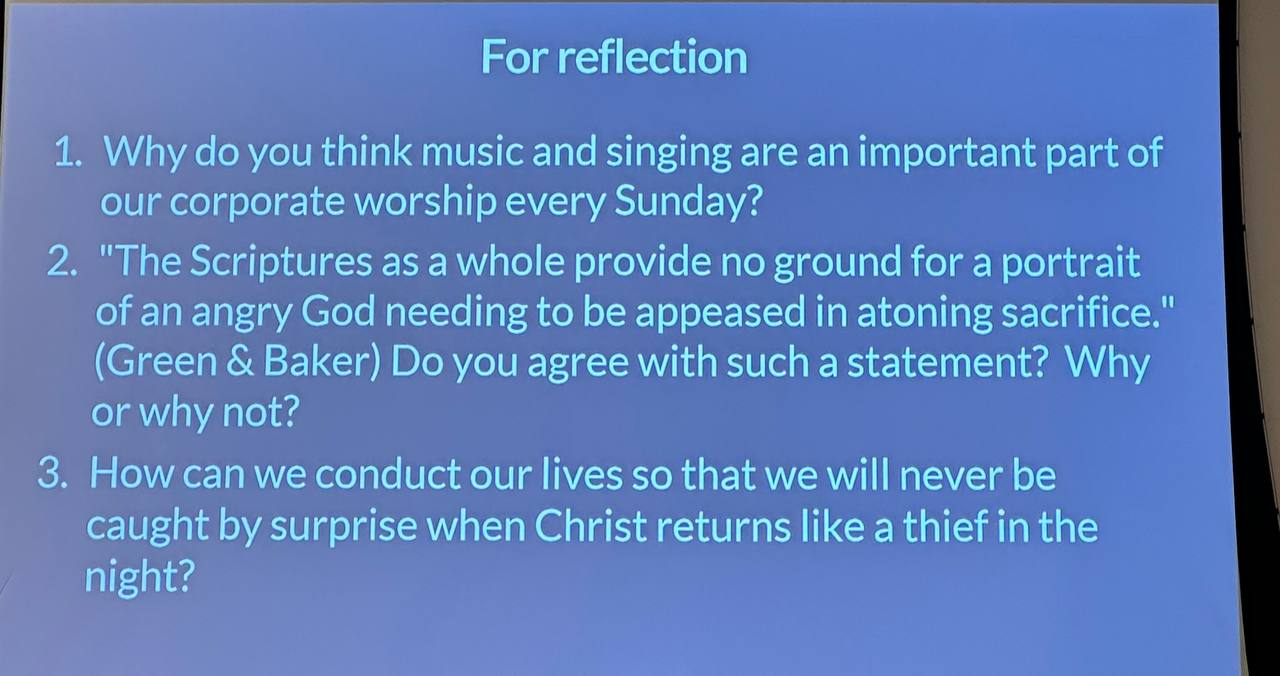
\includegraphics[width=0.8\textwidth, trim={0cm 0cm 0cm 0cm},clip]{Figures/marSermon4Reflections.jpg}
    \caption[]{Reflection questions for this sermon}
    \label{}
  \end{figure}}
\end{itemize}